\chapter{绪论}

\section{研究背景}

\subsection{计算流体力学}

流体力学是物理学的一个分支,
是涉及流体(液体、气体和等离子体)及其作用力的学科。
如同诺贝尔奖获得者威尔逊曾说过的“现代科学研究的三大支柱是科学实验、理论研究、科学计算”,
流体力学分别在这三个方面都有所发展。
在17世纪,
法国和德国开始了实验流体力学的研究。
随后,
在18和19世纪,
欧洲发展起来了理论流体力学。
然后,
随着现代计算机的出现,
第三种重要的方法——计算流体力学(computational fluid dynamics,
CFD)诞生了,
它与纯理论和纯实验研究方法同等重要\upcite{Anderson-CFD}。

与实验手段依靠风洞等实验设施不同的是,
CFD依靠计算机程序,
更加方便、快捷也更加经济。
更重要的是,
CFD可以模拟真实实验室不能揭示的流动现象,
捕捉在特定瞬间的流场状态,
例如观察层流分离流动的不稳定现象;
CFD可以在模拟高超音速流动的同时模拟高温流场,
这是目前的风洞实验做不到的。
但在另一方面,
我们应该也要注意到CFD
依然需要理论流体力学提供理论和模型的支撑,
依然需要实验流体力学提供数据以检验结果,
互相印证。

CFD在预测流体流动方面发挥着重要的作用,
它有许多应用领域,
例如航空航天航海工程、大气科学、环境工程、制造工业等。
当提到CFD使用的数学模型,
不得不提及纳维-斯托克斯方程组和欧拉方程组两个经典模型。
其中,
纳维-斯托克斯方程组是
\begin{equation}
  {\partial_t}
  \begin{bmatrix} \rho \\ \rho {\bm v} \\ \rho E \end{bmatrix}
  +\nabla \cdot
  \begin{bmatrix} \rho {
    \bm v} \\ {\bm v} \otimes (\rho {\bm v})- {\bm\Pi} \\ \rho E{\bm v} - {\bm\Pi}\cdot{\bm v} - \kappa \nabla T\end{bmatrix}
  =
  \begin{bmatrix} 0 \\ \rho {\bm F} \\ \rho {\bm v} \cdot {\bm F} + \rho \dot{q} \end{bmatrix},
\end{equation}
其中,
$\rho$是密度,
${\bm v}$是速度,
$E$是比能量,
比能量满足$E = e + \frac{1}{2} |\bm v|^2$,
$e$是比内能,
$\otimes$是张量积,
${\bm \Pi} = -p \bm I + \bm\tau$是应力张量,
$p$是压强,
$\bm I$是单位向量,
$\bm\tau$是粘性应力张量,
$\kappa$是热导率,
$T$是温度,
$\bm F$是比体积力(例如重力、静电力和洛伦兹力),
$\dot q$是单位时间的比体加热(例如热辐射、电流热效应)。
$\rho$、$e$、$p$和$T$等热力学变量之间满足状态方程,
并且在“热力学平衡”假设下所有热力学变量只有两个自由度,
即所有其他变量均可由这两个自由度表示。
粘性应力张量往往是变形速度张量的函数,
具体关系需要根据具体的流体性质确定。
如果考虑无粘性应力、无热传导的近似情况,
就得到了欧拉方程组
\begin{equation}
  {\partial_t}
  \begin{bmatrix} \rho \\ \rho {\bm v} \\ \rho E \end{bmatrix}
  +\nabla \cdot
  \begin{bmatrix} \rho {
    \bm v} \\ {\bm v} \otimes (\rho {\bm v})+ p \bm I \\ {\bm v}(\rho E+p)\end{bmatrix}
  =
  \begin{bmatrix} 0 \\ \rho {\bm F} \\ \rho {\bm F} \cdot {\bm v} + \rho \dot{q} \end{bmatrix}.
\end{equation}
如果进一步的考虑没有体积力和体加热的情形,
我们有无源的双曲守恒律形式的欧拉方程组
\begin{equation}
  {\partial_t}
  \begin{bmatrix} \rho \\ \rho {\bm v} \\ \rho E \end{bmatrix}
  +\nabla \cdot
  \begin{bmatrix} \rho {
    \bm v} \\ {\bm v} \otimes (\rho {\bm v})+ p \bm I \\ {\bm v}(\rho E+p)\end{bmatrix}
  = 0.
\end{equation}

\subsection{双曲守恒律及其数值格式}

双曲守恒律是形如
\begin{equation}
  \label{eq:balance-law}
  {\partial_t}{\bm u}+\nabla \cdot{\bm f}(\bm u)= 0,
\end{equation}
的方程组,
并且其(在连续意义下等价的)非守恒形式
\begin{equation}
  {\partial_t}{\bm u}+\sum_i{\bm A}_i(\bm u){\partial_{x_i}}\bm u= 0,
\end{equation}
中的系数${\bm A}_i(\bm u)$的特征值都是实数,
这里的$x_i$代表第$i$个空间变量,
例如三维空间中的$x$、$y$和$z$。
对双曲守恒律数值格式的研究工作有很多,
常见的数值格式可以按照网格运动方式、空间离散方法和时间离散方法来分类。

\subsubsection{按照网格运动方式分类}

从网格运动方式上看,
有基于欧拉方法的格式、基于拉格朗日方法的格式和基于任意拉格朗日-欧拉方法的格式。

\begin{figure}[htbp]
  \centering
  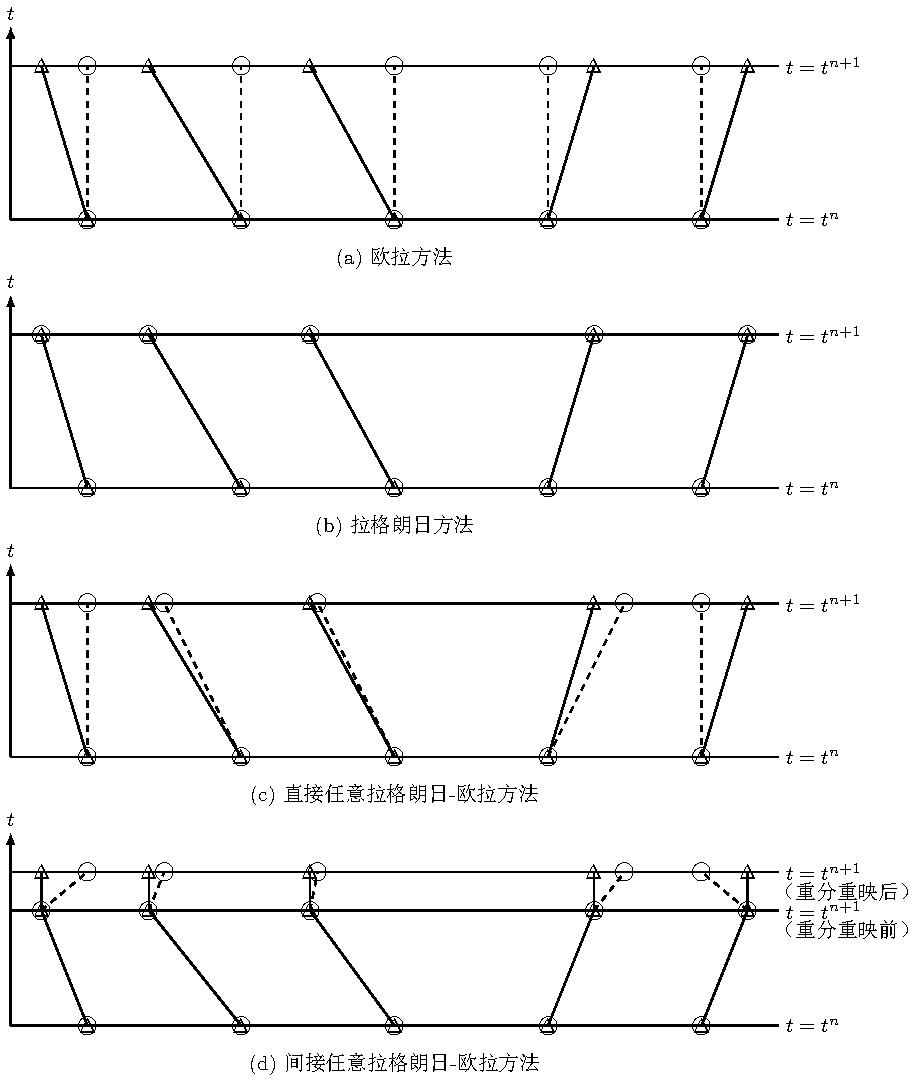
\includegraphics[width=\textwidth]{fig/tikz/EulerLagrange.pdf}
  \caption{四种网格运动方式的示意图。
    $\bigcirc$和虚线代表网格及其运动,
    $\Delta$和实线代表物质及其运动。
  }
  \label{fig:EulerLagrange}
\end{figure}

\begin{enumerate}
  \item 欧拉方法\upcite{GRPpolytropic,AngLi-2023,AngLi-2024}的网格固定不动,
        它比较简单,
        适合处理固定区域和流体变形大的问题,
        例如稳态问题、台阶问题和双马赫反射问题等;
        但是不能追踪质点运动,
        同时在接触间断和物质界面处的耗散大。
  \item 拉格朗日方法\upcite{PP-Lagrange-MM,ENO-Lagrange,qi2018high}的网格节点跟随流体一起运动,
        这种方法在接触间断和物质界面处几乎没有数值耗散,
        能敏锐地捕捉接触间断,
        精确地识别和跟踪物质界面,
        追踪流体运动,
        因此适合处理多介质问题和运动边界问题,
        例如气-水相互作用问题、爆炸问题和活塞问题等。
        但是一般计算比较复杂,
        网格容易变形,
        甚至可能致使计算中止。
        在使用直线网格时,
        拉格朗日方法至多有二阶精度。
  \item 任意拉格朗日-欧拉方法分为直接任意拉格朗日-欧拉方法和间接任意拉格朗日-欧拉方法两种。
        
        直接任意拉格朗日-欧拉方法最早是在文\cite{noh1964cel,franck1964mixed,trulio1966theory,hirt1974arbitrary}中分别提出的\upcite{donea2004arbitrary},
        并在近十年也有许多相关的工作,
        例如文\cite{boscheri2017high,boscheri2014direct,qi2017fully}中的工作。
        这种方法依靠网格移动算法给出网格移动速度,
        并且网格移动速度包含在通量的计算中。
        直接任意拉格朗日-欧拉方法能够保持拉格朗日方法的优势,
        并在处理网格变形大的问题时,
        能够减少计算误差以及避免计算中止;
        不过这种方法需要额外的网格移动算法和网格质量控制算法,
        计算较为复杂。
        前面介绍的欧拉方法可以视为网格移动速度始终为零的特殊情况,
        而拉格朗日方法可以视为网格移动速度与流体速度一致的特殊情况。
        
        间接任意拉格朗日-欧拉方法\upcite{wu2021cell,ReALE}有三步,
        分别是拉格朗日步、网格重分步和物理量重映步。
        在拉格朗日步,
        类似拉格朗日方法更新网格和其上的物理量信息。
        然后在网格重分步,
        根据旧网格和物理量信息,
        计算得到网格质量更好的新网格。
        最后在物理量重映步,
        将旧网格上的物理量信息转移到新网格上。
        这种方法也能够保持拉格朗日方法的优势,
        并在处理网格变形大的问题时,
        能够减少计算误差以及避免计算中止。
        与直接任意拉格朗日-欧拉方法不同的是,
        间接任意拉格朗日-欧拉方法不需要设计复杂的网格移动算法;
        但是需要设计网格重分和物理量重映算法。
\end{enumerate}

\subsubsection{按照空间离散方法分类}

从空间离散方法上看,
可以归类为有限差分、有限体积和间断有限元格式。

\begin{enumerate}
  \item 有限差分格式\upcite{sod1978survey,zhang2023fifth}在一系列离散点上储存和更新变量,
        相对易于实现,
        简单高效,
        特别适用于均匀和光滑的结构网格;
        但是难以处理复杂的几何区域,
        对网格的光滑性要求较高。
  \item 有限体积格式\upcite{eymard2000finite,zhu2016new}是将计算区域分割为一系列控制体,
        在这些控制体上储存和更新变量,
        相对而言它更灵活,
        可以更方便地处理非结构网格以及非规则区域,
        并且很容易满足守恒性;
        然而计算成本相对较高。
  \item 间断有限元格式\upcite{cockburn1998DG,cockburn1991runge}也同样在控制体上储存变量,
        不过储存的是多项式。
        它的显式格式在一次推进中,
        除了需要相邻单元提供每个边界外侧流入的通量之外,
        不使用其他控制体的信息。
        间断有限元格式可以方便的处理非结构网格和复杂的几何形状,
        很容易满足守恒性,
        得到的格式一般更加紧致;
        不过一般时间步长较小,
        导致计算成本很高。
\end{enumerate}

\subsubsection{按照时间离散方法分类}

从时间离散方法上看,
分为显式、隐式和显隐式格式。

\begin{enumerate}
  \item 显式格式\upcite{du2018hermite,AngLi-2023,AngLi-2024}的空间离散只使用本时间层以及更早的时间层的已知量,
        因而可以直接将下一层的变量由已知量直接表示出来,
        不需要迭代求解,
        简单高效,
        易于实现;
        但是数值稳定性受限,
        时间步长的选取过大可能导致数值不稳定,
        甚至计算中止。
        时间步长往往要根据Courant-Friedrichs-Lewy(CFL)条件选取,
        并随着网格尺度的减小而减小,
        同时也会随着问题的刚性强度增大而减小。
        所以,
        显式格式不太适合计算强刚性问题。
  \item 隐式格式\upcite{beam1976implicit,mulder1985experiments}的空间离散使用待求时间层的未知量,
        这导致未知量耦合在一起,
        需要求解方程组,
        方程组的规模随着网格加密而增加,
        这给计算和存储都带来了很大的困难。
        如果涉及非线性问题还需要迭代求解非线性方程组,
        求解比较复杂,
        导致单个时间步的计算开销较大。
        不过有数值稳定性好、能够处理强刚性问题和较大的时间步长带来的整体开销可能较小等优点。
  \item 显隐式格式\upcite{arun2020asymptotic,tan2022stability}将前两者结合在一起,
        通过对方程适当的分解,
        显式离散非刚性项,
        隐式离散强刚性项,
        得到一个结合了显式和隐式优点的显隐式格式。
        显隐式格式可以扬长避短,
        隐式离散强刚性项可以选择较大的时间步长,
        从而降低计算开销。
        当刚性项是线性的时候,显式离散非线性非刚性项可以避免求解非线性代数方程组,
        降低了求解方程组的难度,
        并进一步的降低了计算开销。
        当刚性项是非线性的时候,
        可以使用explicit-implicit-null(EIN)技术\upcite{tan2022stability,duchemin2014explicit,wang2020local}将刚性项${\partial_x} {\bm f}({\bm u})$分解为一个非线性弱刚性项和一个线性强刚性项,
        即
        \begin{equation}
          {\partial_x} {\bm f}({\bm u}) = {\partial_x} \left({\bm f}({\bm u})-{\bm A}u\right) + {\partial_x} \left({\bm A}{\bm u}\right),
        \end{equation}
        其中,
        ${\bm A}u$是${\bm f}({\bm u})$的局部线性化近似。
        然后分别用显式和隐式格式求解两项。
        但是显隐式格式的设计成本略高于显式和隐式格式。
\end{enumerate}

\section{研究现状}

近些年,
CFD应用对精确模拟流体流动状态的需求,
推动了对高精度格式的需求。
然而,
对高精度的追求必须与计算成本相权衡,
这使得设计一个高精度高效的数值格式成为一个有趣且具有挑战性的问题。
此外,
为了更准确地捕捉流场中的细节,
例如湍流和激波,
我们需要开发高分辨率的格式,
这可以通过构造更加紧致的格式来实现。
同时,
使用更加紧致的格式可以有效地减少计算节点之间的通信开销,
在并行计算中更加高效。

因此,
本文将致力于研究求解双曲守恒律的高精度紧致数值格式,
具体地说,
本文将致力于研究基于欧拉框架的显式有限体积格式。
这个数值格式通常可以分成三个部分:时间推进框架、重构算法和解法器。
对于一维情形下的双曲守恒律 \cref{eq:balance-law},
我们定义计算单元$I_i$上的单元平均值为
\begin{equation}
  \bar{\bm{u}}_{i}(t)=\frac{1}{h}\int_{I_{i}} {\bm{u}}(x,t) dx,
\end{equation}
则有
\begin{equation}
  \frac{d \bar{\bm{u}}_i(t)}{dt} = \mathcal{L}({\bm{u}}_i) \triangleq -\frac{1}{h} \left({\bm{f}}({\bm{u}}(x_{i+\frac 12},t)) - {\bm{f}}({\bm{u}}(x_{i-\frac 12},t))\right),
\end{equation}
接着我们得到了近似的半离散形式
\begin{equation}
  \label{eq:semi-uniform}
  \frac{d \bar{\bm{u}}_i(t)}{dt} = \hat{\mathcal{L}}({\bm{u}}_i) \triangleq -\frac{1}{h} \left(\hat{\bm{f}}({\bm{u}}_{i+\frac 12,-},{\bm{u}}_{i+\frac 12,+}) - \hat{\bm{f}}({\bm{u}}_{i-\frac 12,-},{\bm{u}}_{i-\frac 12,+})\right).
\end{equation}
一般地,
为了得到数值通量$\hat{\bm{f}}({\bm{u}}_{i+\frac 12,-},{\bm{u}}_{i+\frac 12,+})$,
需要使用重构算法和解法器。
在某个时间层,
重构算法根据单元平均值$\bar{\bm{u}}_{i}$等信息重构出一个多项式,
再由多项式给出在单元边界处空间中某个方向上的近似值${\bm u}_{i+\frac{1}{2},\pm}$。
然后解法器根据重构的结果,
给出在单元边界处的数值通量$\hat{\bm{f}}({\bm{u}}_{i+\frac 12,-},{\bm{u}}_{i+\frac 12,+})$。
时间推进框架则是利用重构算法和解法器给出的数值通量,
从初始时刻依次得到每个时间层的单元平均值,
直到时间终点。
下面将分别从时间推进框架、重构算法和解法器这三部分,
介绍求解双曲守恒律的基于欧拉框架的显式有限体积格式的研究现状。

\subsection{时间推进框架}

可以根据文\cite{MSMD}中的分类方法,
将常见的时间推进框架分为四类。

\begin{enumerate}
  \item 单步单导数(single-stage single-derivative,
        SSSD)方法,
        也就是欧拉向前方法\upcite{torobook},
        这是出现最早的时间推进框架。
        单步方法是指只使用一次时间推进就可以得到下一个时间层的单元平均值。
        单导数方法最初是指求解常微分方程时,
        只使用函数的一阶导数的数值方法;
        相对应的有多导数方法,
        不只使用函数的一阶导数,
        还使用高阶导数来提高计算的精度和效率。
        在处理偏微分方程时,
        可以将相应的概念推广到时间推进中,
        单导数方法是采用如下的时间离散:
        \begin{equation}
          \bar{\bm{u}}_i^{n+1} = \bar{\bm{u}}_i^{n} + \tau \frac{d \bar{\bm{u}}_i(t^n)}{dt} = \bar{\bm{u}}_i^{n} + \tau \mathcal{L}({\bm{u}}_i^n),
        \end{equation}
        其中,
        $\bar{\bm{u}}_i^{n}$是时间层$t^n$的单元平均值,
        $\tau=t^{n+1}-t^n$是时间步长。
        采用适当的重构算法和解法器可以得到$\mathcal{L}({\bm{u}}_i^n)$的数值近似$\hat{\mathcal{L}}({\bm{u}}_i^n)$,
        并得到如下推进形式:
        \begin{equation}
          \label{eq:euler-forward}
          \bar{\bm{u}}_i^{n+1} = \bar{\bm{u}}_i^{n} + \tau \hat{\mathcal{L}}({\bm{u}}_i^n),
        \end{equation}
        这是一个一阶精度的时间推进框架,
        以此为基础发展出来了下面许多种高精度时间推进框架。
  \item 多步单导数(multi-stage single-derivative,
        MSSD)方法,
        例如:龙格库塔(Runge-Kutta,
        RK)方法,
        最早由Carl Runge和Wilhelm Kutta于1900年左右提出,
        并用于求解常微分方程。
        后来有许多将之用于偏微分方程求解的工作\upcite{VANDERHOUWEN1996261}。
        然后,
        文\cite{SSP-2011}中提出了强稳定保持的龙格库塔(strong-stability preserving Runge-Kutta,
        SSP-RK)方法,
        这是一系列方法,
        其中一个广泛使用的是三阶精度的SSP-RK方法,
        它通过三个时间层(包括两个中间时间层${\bm{u}}^{(1)}$和${\bm{u}}^{(2)}$)可以得到时间方向上三阶精度的近似:
        \begin{align}
          \bar{\bm{u}}_i^{(1)} & = \bar{\bm{u}}_i^{n} + \tau \hat{\mathcal{L}}(\bar{\bm{u}}_i^{n})                                                               \\
          \bar{\bm{u}}_i^{(2)} & = \frac{3}{4} \bar{\bm{u}}_i^n + \frac{1}{4} \left(\bar{\bm{u}}_i^{(1)} + \tau \hat{\mathcal{L}}(\bar{\bm{u}}_i^{(1)})\right)   \\
          \bar{\bm{u}}_i^{n+1} & = \frac{1}{3} \bar{\bm{u}}_i^n + \frac{2}{3} \left(\bar{\bm{u}}_i^{(2)} + \tau \hat{\mathcal{L}}(\bar{\bm{u}}_i^{(2)})\right).
        \end{align}
        这种方法还是一种单导数方法,
        因为只用到了$\hat{\mathcal{L}}({\bm{u}})$来近似一阶导数${d \bar{\bm{u}}_i(t)}/{dt}$,
        即$\mathcal{L}({\bm{u}})$。
        不过由于引入了中间时间层,
        这是一个多步方法。
        SSP-RK方法可以表达为欧拉向前方法 \cref{eq:euler-forward} 的凸组合,
        并因此可以较为容易的推导出包括保正\upcite{PP-Lagrange-MM}在内的许多良好性质;
        不过由于数个中间时间层的存在,
        最终得到的数值格式往往不太紧致。
  \item 单步多导数(single-stage multi-derivative,
        SSMD)方法,
        例如:拉克斯-温德洛夫(Lax-Wendroff,
        LW)方法\upcite{Lax-Wendroff}及其三阶和四阶的拓展\upcite{LW3-LW4},
        这类方法不需要多个中间时间层来达到高阶精度,
        而是引入了高阶导数项,
        例如一步三阶的LW方法采用如下的时间离散
        \begin{equation}
          \bar{\bm{u}}_i^{n+1} = \bar{\bm{u}}_i^{n} + \tau \frac{d \bar{\bm{u}}_i(t^n)}{dt} + \frac{\tau^2}{2} \frac{d^2 \bar{\bm{u}}_i(t^n)}{dt^2} + \frac{\tau^3}{6} \frac{d^3 \bar{\bm{u}}_i(t^n)}{dt^3} = \bar{\bm{u}}^n + \tau \mathcal{L}(\bar{\bm{u}}^{n}) + \frac{\tau^2}{2} {\partial_t}\mathcal{L}(\bar{\bm{u}}^{n}) + \frac{\tau^3}{6} {\partial_t^2}\mathcal{L}(\bar{\bm{u}}^{n}),
        \end{equation}
        采用适当的重构算法和解法器可以得到$\mathcal{L}(\bar{\bm{u}}_i^n)$、${\partial_t}\mathcal{L}(\bar{\bm{u}}_i^n)$和${\partial_t^2}\mathcal{L}(\bar{\bm{u}}_i^n)$的数值近似$\hat{\mathcal{L}}(\bar{\bm{u}}_i^n)$、$\widehat{{\partial_t}\mathcal{L}}(\bar{\bm{u}}_i^n)$和$\widehat{{\partial_t^2}\mathcal{L}}(\bar{\bm{u}}_i^n)$,
        并得到如下推进形式:
        \begin{equation}
          \bar{\bm{u}}_i^{n+1} = \bar{\bm{u}}_i^n + \tau \hat{\mathcal{L}}(\bar{\bm{u}}_i^{n}) + \frac{\tau^2}{2} \widehat{{\partial_t}\mathcal{L}}(\bar{\bm{u}}_i^{n}) + \frac{\tau^3}{6} \widehat{{\partial_t^2}\mathcal{L}}(\bar{\bm{u}}_i^n).
        \end{equation}
        其中$\widehat{{\partial_t}\mathcal{L}}(\bar{\bm{u}}_i^n)$和$\widehat{{\partial_t^2}\mathcal{L}}(\bar{\bm{u}}_i^n)$需要通过类似文\cite{Qiu-Shu-2003,Qian,Yang}中的三阶LW型解法器获得。
        这样的时间推进方法是多导数方法,
        因为不只使用一阶导数,
        还使用高阶导数。
        SSMD方法得到的格式更加紧致;
        但是高阶导数的引入导致了算法很复杂,
        使得公式和编程都变得复杂,
        尤其当求解高维方程组的时候,
        需要求解相应的Jacobi矩阵。
  \item 多步多导数(multi-stage multi-derivative,
        MSMD)方法\upcite{MSMD,Seal-2016}。
        MSSD方法中过多的中间时间层会使得数值格式不紧致,
        SSMD方法中高阶导数会使得数值格式很复杂,
        MSMD方法结合了这两种方法,
        是数值格式的紧致性和复杂性之间的一种权衡。
        MSMD方法往往只使用一阶和二阶导数,
        同时加入一到两个中间时间层,
        常见的有两步四阶方法和三步五阶方法。
        近十年有许多与两步四阶方法相关的工作,
        例如文\cite{li2016two,Pan-2016,S2O4_wenli}。
        两步四阶方法的推进形式为
        \begin{align}
          \bar{\bm{u}}_i^{*}   & = \bar{\bm{u}}_i^n + \frac{\tau}{2} \hat{\mathcal{L}}(\bar{\bm{u}}_i^{n}) + \frac{\tau^2}{8} \widehat{{\partial_t}\mathcal{L}}(\bar{\bm{u}}_i^{n})                                                                                   \\
          \bar{\bm{u}}_i^{n+1} & = \bar{\bm{u}}_i^n + \tau \hat{\mathcal{L}}(\bar{\bm{u}}_i^{n}) + \frac{\tau^2}{2} \left(\frac{1}{3}\widehat{{\partial_t}\mathcal{L}}(\bar{\bm{u}}_i^{n}) +\frac{2}{3}\widehat{{\partial_t}\mathcal{L}}(\bar{\bm{u}}_i^{*})\right).
        \end{align}
        MSMD方法权衡了数值格式的紧致性和复杂性,
        得到的数值格式的紧致性和复杂性均介于MSSD和SSMD两个方法之间。
        由于两步四阶方法不能表示为一步两阶方法的凸组合,
        一步两阶方法的良好性质的无法直接推广到两步四阶方法上。
\end{enumerate}

\subsection{重构算法}

根据文\cite{PNPM}中的分类方法,
可以将常见的有限体积重构算法归类到$P_NP_M$方法中,
其中,
$N$是指每个单元内的数据所表示的多项式次数,
$M$是边界点值重构时所用的多项式次数。
这样的重构算法往往有$M$阶精度。

\subsubsection{$P_0P_k$方法}

$P_0P_k$方法有基本无振荡(essentially non-oscillatory,
ENO)重构\upcite{ENO-1987}、加权基本无振荡(weighted ENO,
WENO)重构\upcite{WENO,WENO-1994,WENO-1996,WENO-2020,WENOonTRI}、WENO-Z重构\upcite{WENO_Z}、中心型WENO(central WENO,
CWENO)重构\upcite{CWENO-origin,CWENO13579}以及阶数自适应WENO(WENO with adaptive order,
WENO-AO)重构\upcite{WENOAO}等。

这些重构在每个单元内只有一个数据——单元平均值,
然后结合相邻单元中的数据可以得到多项式函数空间$\mathcal{P}^k$中的重构多项式。
ENO重构通过选择附近所有大小为$k$的候选模板中最光滑的模板来尽可能避免振荡;
然而,
这种方法忽略了来自其他模板的有价值的数据。
作为其改进版本,
WENO重构在光滑区域内接受所有模板以获得更高阶精度,
同时通过合理地选取光滑因子和非线性权,
保留了尽可能避免振荡的能力。
在五阶精度的WENO重构中,
光滑因子选取为
\begin{equation}
  \beta_r= \sum_{d=1}^3 \int_{I_{i}}h^{2\ell-1}\left({\partial_{x}^{d}}p_{i}^{(r)}(x)\right)^2 dx,
  \quad r=0,1,2,
\end{equation}
其中,
$\beta_{{r}}$是光滑因子,
$h$是单元$I_i$的大小,
以及$p_{i}^{(r)}(x)$是第$r$个模板的重构多项式。
非线性权选取为
\begin{equation}
  \omega_{{r}}=\frac{\alpha_{{r}}}{\sum_{s=0}^{2}\alpha_{{s}}}, \quad
  \alpha_{{r}}=\frac{\gamma_{{r}}}{\left(\varepsilon+\beta_{{r}}\right)^2}, \quad {{r}}=0,1,2,
\end{equation}
其中,
$\omega_{{r}}$是非线性权,
$\gamma_{{r}}$是线性权,
以及$\varepsilon$是一个小量。
WENO-Z、CWENO和WENO-AO重构通过进一步的改进模板和非线性权的选择策略,
分别取得了一些在特定情形下的良好性能。
例如五阶的WENO-Z重构不再使用原始五阶WENO重构中的非线性权,
而是采用了如下的非线性权
\begin{equation}
  \omega_{{r}}=\frac{\alpha_{{r}}}{\sum_{s=0}^{2}\alpha_{{s}}}, \quad
  \alpha_{{r}}=\gamma_{{r}}\left( 1+\left( \frac{\theta}{\beta_{{r}}+\varepsilon}\right)^q \right) , \quad {{r}}=0,1,2,
\end{equation}
其中,
$\theta = |\beta_{0}-\beta_{2}|$。
这样的改动能够改善原始WENO重构对应的数值格式在极值点处的掉阶问题;
不过$\theta$的构造方式可能难以推广。
CWENO和WENO-AO重构不再选择附近所有大小为$k$的模板作为模板组份,
而是选择了一系列不同大小的模板。
例如,
文\cite{CWENO13579}中选择了大小为1、3、5、7和9的模板作为模板组份,
并得到了一阶、三阶、五阶、七阶和九阶的CWENO格式。
这样的选择使得不能按照原始WENO重构的方法找到线性权,
在文\cite{WENOAO}中给出了这个困难的解决方法。

\subsubsection{$P_1P_k$方法}

作为$P_1P_k$方法的代表,
埃尔米特加权基本无振荡(Hermite WENO,
HWENO)重构\upcite{Qiu-Shu-2004,Qiu-Shu-2005}的每个单元不止含有单元平均值,
还有导数平均值,
这使得相同精度阶数的情况下,
HWENO重构有相比于WENO重构更窄的模板,
因而得到的数值格式会更加紧致。
例如,
同样是一维情形下的五阶重构,
一个WENO重构多项式总计使用了附近5个单元的信息,
而一个HWENO重构多项式仅使用附近3个单元的信息,
如\cref{fig:HWENO} 所示。
$P_1P_k$方法也是两步四阶时间推进框架中所要求的两值格式。

\begin{figure}[htbp]
  \centering
  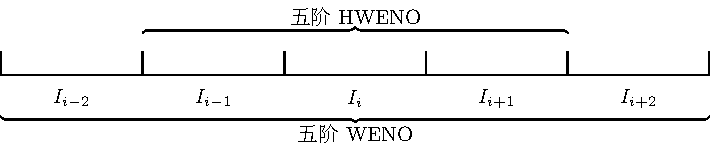
\includegraphics{fig/tikz/HWENO.pdf}
  \caption{一维情形下的五阶WENO重构和五阶HWENO重构模板大小的示意图。
  }
  \label{fig:HWENO}
\end{figure}

另外,
$\mathcal{P}^1$ 间断有限元(discontinuous Galerkin,
DG)方法\upcite{DG-1989,DG-1990,DG-2016}的空间离散,
也是$P_1P_k$方法,
其中,
$k=1$。

\subsubsection{$P_kP_k$方法}

经典的DG方法\upcite{DG-1989,DG-1990,DG-2016}的空间离散也可以视作重构算法,
属于$P_kP_k$方法,
其重构多项式就是每个单元内部储存的多项式,
因而实际上无需做重构运算。

\subsubsection{$P_NP_M$方法}

除了上述这些重构之外,
还有一系列被称为埃尔米特DG或者$P_NP_M$ DG的格式使用了$P_NP_M$方法。
例如文\cite{PNPM}中使用了至多三维的并且$N$和$M$满足$0\le N \le M\le 6$的所有$P_NP_M$方法。
在文\cite{luo2012hermite,xia2014implicit}中使用$P_1P_2$方法。
以$P_1P_2$方法为例,
它在每个单元内储存的自由度可以表示$\mathcal{P}^1$空间中的一个多项式,
然而在自由度的时间推进中使用了二次多项式($\mathcal{P}^2$空间),
这是借助相邻单元中的自由度重构得到的。

\subsection{解法器}

1959年,
Godunov在文\cite{godunov}中提出了利用黎曼问题的解近似单元边界处的通量,
这种方法被称为Godunov解法器。
具体地,
如果重构算法给出了单元边界两侧的近似值${\bm u}_{i+\frac{1}{2},\pm}$,
那么在这个单元边界处对应了一个黎曼问题
\begin{equation}
  \label{eq:RP}
  \left\{
  \begin{aligned}
     & {\partial_{t}}{\bm{u}} + {\partial_{x}}{\bm{f}}({\bm{u}}) = 0, \\
     & {\bm{u}}(x,0) =
    \begin{cases}
      {\bm u}_{i+\frac{1}{2},-}, & x<x_{i+\frac{1}{2}},  \\
      {\bm u}_{i+\frac{1}{2},+}, & x>x_{i+\frac{1}{2}}.
    \end{cases}
  \end{aligned}
  \right.
\end{equation}

欧拉方程组黎曼问题的一个典型的波系结构如\cref{fig:RP_wave_pattern} 所示。
如果这个黎曼问题的精确解是${\bm{u}}(x,t)={\bm R}(x/t;{\bm u}_{i+\frac{1}{2},-},{\bm u}_{i+\frac{1}{2},+})$,
那么Godunov解法器给出的数值通量可以表示为:
\begin{equation}
  \hat{\bm{f}}({\bm{u}}_{i+\frac 12,-},{\bm{u}}_{i+\frac 12,+}) = {\bm R}(0;{\bm u}_{i+\frac{1}{2},-},{\bm u}_{i+\frac{1}{2},+}).
\end{equation}

\begin{figure}[htbp]
  \centering
  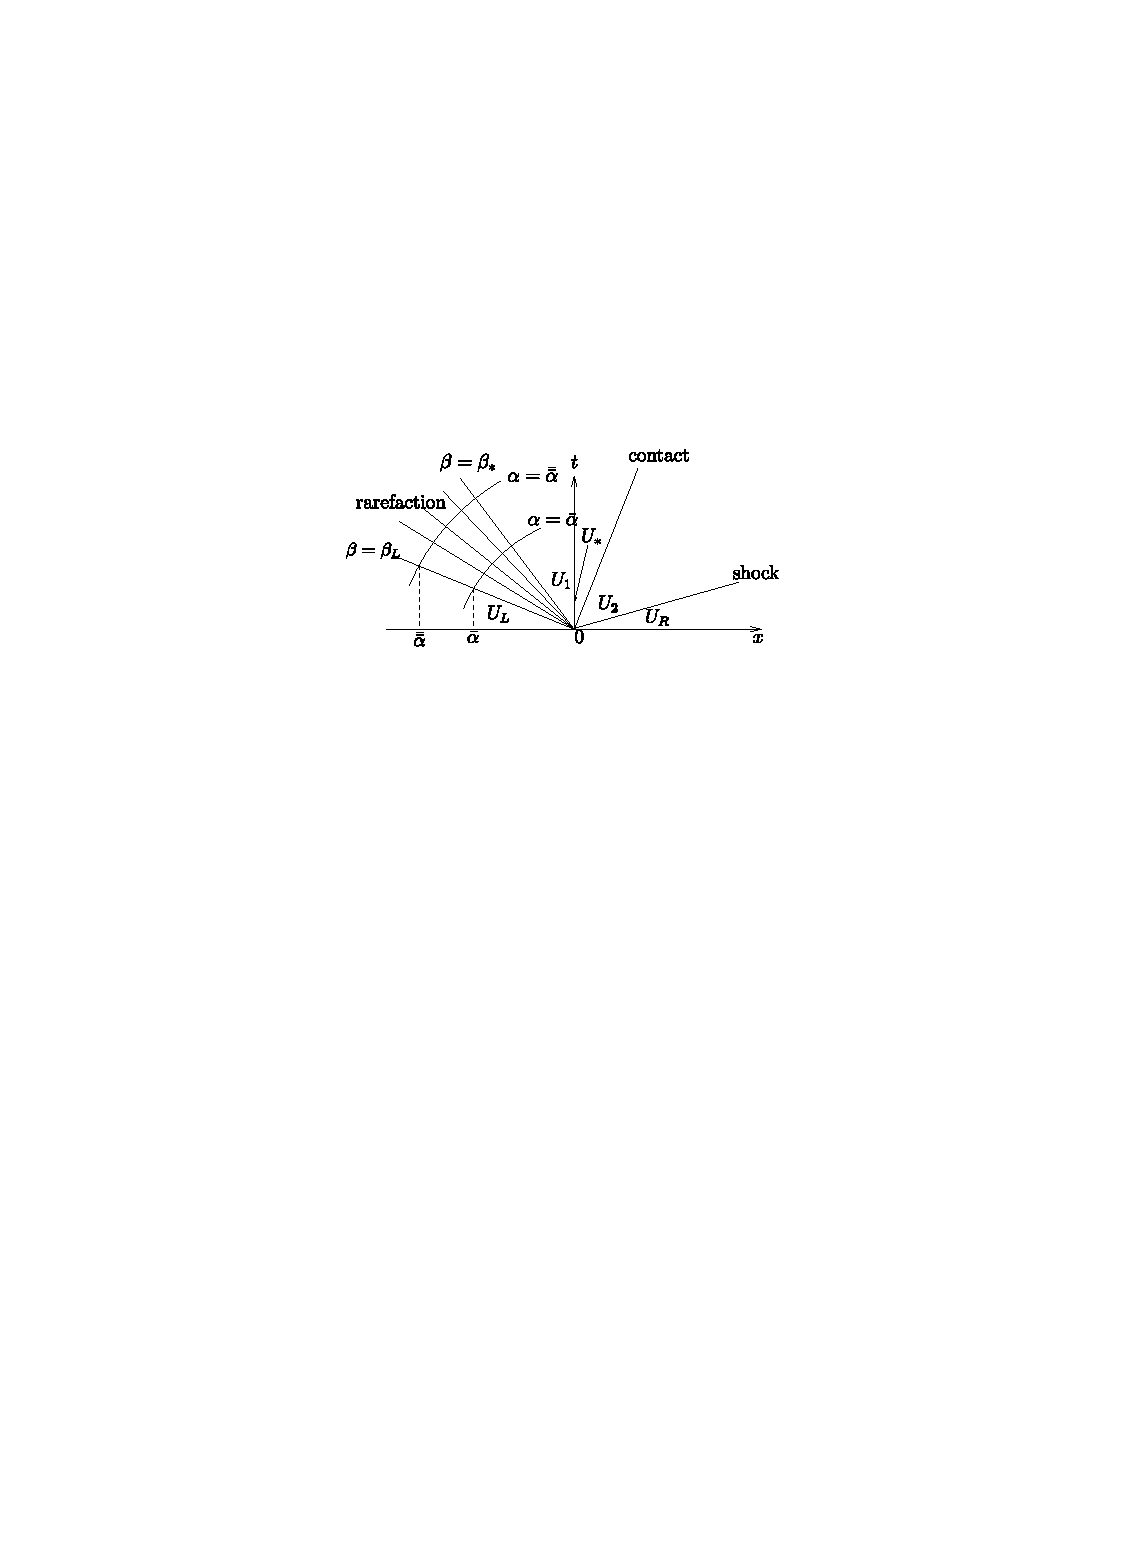
\includegraphics[width=\textwidth]{fig/RP_wave_pattern.pdf}
  \caption{欧拉方程组黎曼问题的一个典型的波系结构示意图。
  }
  \label{fig:RP_wave_pattern}
\end{figure}

除了精确求解黎曼问题外,
还可以使用一些数值近似的方法,
例如Lax-Friedrichs(LF)数值通量是
\begin{equation}
  \hat{\bm{f}}({\bm{u}}_{i+\frac 12,-},{\bm{u}}_{i+\frac 12,+}) = \frac{1}{2}\left(\bm{f}({\bm{u}}_{i+\frac 12,-}) + \bm{f}({\bm{u}}_{i+\frac 12,+}) - \alpha \left({\bm{u}}_{i+\frac 12,+}-{\bm{u}}_{i+\frac 12,-}\right)\right), \quad \alpha = \max_{\bm{u}} \|\bm{f}'(\bm{u})\|.
\end{equation}

局部线性化的Roe解法器\upcite{Roe}则是使用一个局部线性化的矩阵${\bm A}({\bm u}_{i+\frac{1}{2},-},{\bm u}_{i+\frac{1}{2},+})$近似双曲守恒律中的非线性对流项,
得到双曲守恒律的线性近似
\begin{equation}
  {\partial_{t}}{\bm{u}} + {\bm A}({\bm u}_{i+\frac{1}{2},-},{\bm u}_{i+\frac{1}{2},+}){\partial_{x}}{\bm{u}} = 0,
\end{equation}
然后很容易得到这个线性近似方程组的黎曼问题精确解以及相应的数值通量,
进而可以作为原双曲守恒律的一个近似数值通量。
线性近似方程组的黎曼问题的解仅由接触间断和激波构成,
使得这种对稀疏波的近似是非常错误的,
在实际计算中音速点附近会出现非物理的间断\upcite{tang2005sonic},
这需要被称为熵修正的技术\upcite{harten1983self}来处理。

双激波近似的HLL解法器\upcite{HLL}不用考虑双曲守恒律的黎曼问题的实际波系结构情况,
均利用双激波结构近似。
通过适当的波速估计算法直接给出两个激波的速度,
就可以很容易得到近似波系结构下的黎曼问题精确解以及相应的数值通量,
进而可以作为原双曲守恒律的一个近似数值通量。
HLL通量在只有两个方程的情况下,
是稳健的近似黎曼问题解法器,
不过对于欧拉方程组等有更多变量的方程组而言,
这种假设是不对的,
会导致接触间断和物质界面的分辨率低下。

针对HLL解法器存在的问题,
通过在近似波系结构中添加一个接触间断,
得到了双激波单接触间断近似的HLLC解法器\upcite{HLLC},
这种解法器可以较好的近似欧拉方程组等多变量方程组。
除了上述这些解法器,
还有许多近似黎曼问题解法器,
这里不再一一列出。

在1984年,
Ben-Artzi等人在文\cite{GRPgeneral}中提出了广义黎曼问题解法器,
用于一个基于拉格朗日框架的二阶精度数值格式。
随后文\cite{GRPpolytropic}的作者推广了该解法器,
使其可以直接用于基于欧拉框架的数值格式。
然后,
该解法器又被进一步推广,
使其可以应用于任意气体状态方程\upcite{GRP}。
这种解法器要求重构不只要提供函数近似值${\bm u}_{i+\frac{1}{2},\pm}$,
还需要提供导数近似值$\left({\partial_x}{\bm u}\right)_{i+\frac{1}{2},\pm}$,
那么在这个单元边界处对应了一个广义黎曼问题
\begin{equation}
  \label{eq:GRP}
  \left\{
  \begin{aligned}
     & {\partial_{t}}{\bm{u}} + {\partial_{x}}{\bm{f}}({\bm{u}}) = 0, \\
     & {\bm{u}}(x,0) =
    \begin{cases}
      {\bm u}_{i+\frac{1}{2},-} + \left({\partial_x}{\bm u}\right)_{i+\frac{1}{2},-} x, & x<x_{i+\frac{1}{2}},  \\
      {\bm u}_{i+\frac{1}{2},+} + \left({\partial_x}{\bm u}\right)_{i+\frac{1}{2},+} x, & x>x_{i+\frac{1}{2}},
    \end{cases}
  \end{aligned}
  \right.
\end{equation}
而不再是原来的黎曼问题 \cref{eq:RP}。

欧拉方程组广义黎曼问题的一个典型的波系结构如\cref{fig:GRP_wave_pattern} 所示。
在广义黎曼问题解法器求解这个广义黎曼问题时,
由于方程组的非线性,
我们往往难以得到 \cref{eq:GRP} 的解${\bm{u}}(x,t)$的全部信息,
而是得到两个近似值${\bm{u}}_{i+\frac{1}{2}}^{n,+}$和$\left({\partial_{t}}{\bm{u}}\right)_{i+\frac{1}{2}}^{n,+}$,
它们满足(或近似地满足)
\begin{equation}
  \label{eq:limit}
  {\bm{u}}_{i+\frac{1}{2}}^{n,+} = \lim_{t\to t^n,+} {\bm{u}}(x_{i+\frac{1}{2}},t), \quad
  \left({\partial_{t}}{\bm{u}}\right)_{i+\frac{1}{2}}^{n,+} = \lim_{t\to t^n,+} {\partial_{t}}{\bm{u}}(x_{i+\frac{1}{2}},t).
\end{equation}
注意,
这里的${\bm{u}}_{i+\frac{1}{2}}^{n,+}$是通过一个黎曼问题解法器得到的,
如果是近似的黎曼问题解法器,
那么 \cref{eq:limit} 中的两个关系都是近似满足的。
对于$\left({\partial_{t}}{\bm{u}}\right)_{i+\frac{1}{2}}^{n,+}$,
广义黎曼问题解法器有精确求解的非线性版本和声波近似的版本,
如果采用的是声波近似的版本,
那么 \cref{eq:limit} 中的第二个关系就是近似满足的。
如果采用的是精确的黎曼问题解法器和非线性版本的广义黎曼问题解法器,
那么 \cref{eq:limit} 中的两个关系就都是精确满足的。
接下来,
广义黎曼问题解法器给出的数值通量可以表示为:
\begin{equation}
  \hat{\bm{f}}({\bm{u}}_{i+\frac 12,-},{\bm{u}}_{i+\frac 12,+},\left({\partial_x}{\bm u}\right)_{i+\frac{1}{2},-},\left({\partial_x}{\bm u}\right)_{i+\frac{1}{2},+}) = {\bm{f}}\left({\bm{u}}_{i+\frac{1}{2}}^{n,+}\right) + \frac{\tau}{2} \frac{\partial{\bm{f}}}{\partial{\bm{u}}}\left({\bm{u}}_{i+\frac{1}{2}}^{n,+}\right) \left({\partial_{t}}{\bm{u}}\right)_{i+\frac{1}{2}}^{n,+}.
\end{equation}

\begin{figure}[htbp]
  \centering
  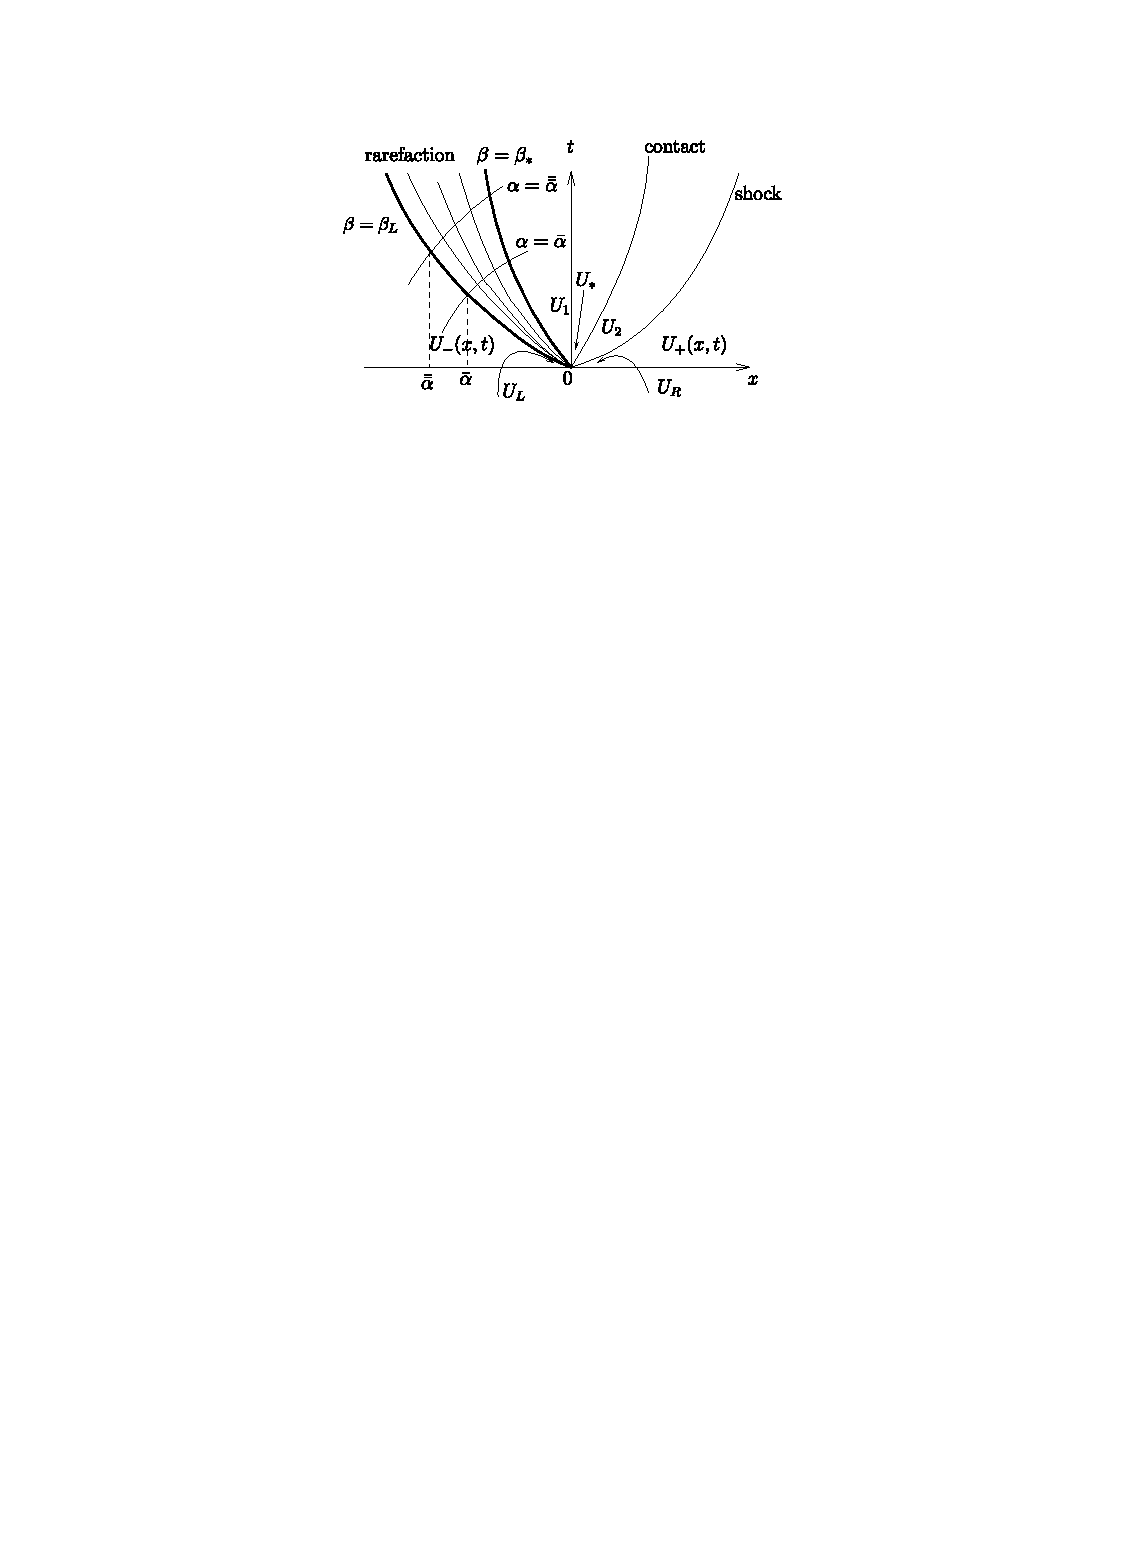
\includegraphics[width=\textwidth]{fig/GRP_wave_pattern.pdf}
  \caption{欧拉方程组广义黎曼问题的一个典型的波系结构示意图。
  }
  \label{fig:GRP_wave_pattern}
\end{figure}

二维情形下的广义黎曼问题解法器可以参考文\cite{GRP_qi}中的二维弱耦合的广义黎曼问题解法器。

\vspace{\baselineskip} % 属于节的内容
采用了埃尔米特重构的两步四阶时间推进框架往往有两种做法,
一种是文\cite{Qiu-Shu-2004,S2O4_wenli}使用的做法,
对双曲守恒律 \cref{eq:balance-law} 求导得到
\begin{equation}
  \label{eq:diff-balance}
  {\partial_t}{\bm v}+\nabla \cdot{\bm g}(\bm u, \bm v)= 0, \quad
  \bm v(x)={\partial_x}\bm u(x),\quad
  \bm g(\bm u, \bm v)={\bm f}'({\bm u}) \ {\bm v}.
\end{equation}
然后分别对 \cref{eq:balance-law,eq:diff-balance} 采取两步四阶离散。

另一种做法是文\cite{li2016two}中提出的时间推进框架,
利用了牛顿-莱布尼茨公式直接得到了一个与双曲守恒律 \cref{eq:balance-law} 无关的,
关于导数${\bm v}(x)={\partial_x}\bm u(x)$在单元$(x_{i-\frac{1}{2}},x_{i+\frac{1}{2}})$上平均值$\bar{\bm v}_i$的恒等式
\begin{equation}
  \bar{\bm v}_i =\frac{1}{x_{i+\frac{1}{2}} -  x_{i-\frac{1}{2}}}\int_{x_{i-\frac{1}{2}}}^{x_{i+\frac{1}{2}}} v(x) dx= \frac{u(x_{i+\frac{1}{2}}) -  u(x_{i-\frac{1}{2}})}{x_{i+\frac{1}{2}} -  x_{i-\frac{1}{2}}},
\end{equation}
然后可以基于此式与LW型解法器推进导数平均值,
具体的细节可以参考\cref{sec:framework}。
在本文,
我们约定下文再次提及的两步四阶时间推进框架将会是特指文\cite{li2016two}中提出的时间推进框架,
它是一个使用了埃尔米特重构和LW型解法器的时间推进框架,
这与文\cite{Qiu-Shu-2004,S2O4_wenli}中的做法是不同的。

\section{本文的研究目的和主要工作}

文\cite{du2018hermite}中作者针对双曲守恒律,
基于五阶精度HWENO(HWENO5)和五阶精度WENO(WENO5)重构以及广义黎曼问题解法器,
设计了一种两步四阶数值格式。
这种数值格式有一维和二维两个版本,
其中二维采用的重构是逐维的。
具体来说,
在一维情形下,
该格式使用HWENO5重构来获得单元边界上的函数值,
并使用WENO5重构来获得导数值。
在二维情形下,
逐维地使用HWENO5重构来获得单元边界上的函数值,
并在两个空间方向上分别使用WENO5和HWENO5重构来获得导数值。

为了进一步提高数值格式的紧致性,
本文致力于研究求解双曲守恒律的基于紧致埃尔米特重构的显式两步四阶有限体积格式,
即函数值和导数值均使用埃尔米特重构获得。
同时希望时空均是四阶精度的。
此外在二维情形下,
逐维重构方法不能保证对称性,
内存需求较高,
因为需要两次扫描网格并存储中间变量,
并且很难推广到非结构网格。
所以,
我们要构造一个真正的二维重构,
并设计相应的两步四阶格式。

我们首先提出了改进的两步四阶时间推进框架。
在本文我们旨在分别设计一维与二维时空四阶精度基本无振荡的两步四阶格式。
具体的,
在一维情形下,
我们先构造一种四阶埃尔米特重构,
其比WENO5和HWENO5重构更加紧致,
计算开销更小。
然后在原始的两步四阶时间推进框架中采用这种新构造的重构,
并希望能够得到时空四阶精度基本无振荡的两步四阶格式。
然而我们发现原始的两步四阶时间推进框架的紧致性和高精度不可兼得。
如果导数重构采用更加紧致的埃尔米特重构,
那么所得格式在光滑区域的精度只有三阶精度。
随后,
我们分析了其原因,
并分别在一维和二维两种情形下提出了改进的两步四阶时间推进框架。
在改进的框架中导数重构采用更加紧致的埃尔米特重构时,
获得的数值格式可以在光滑区域保持四阶精度。

接着,
我们设计了一维基于紧致埃尔米特重构的双曲守恒律基本无振荡的两步四阶数值格式。
具体地说,
在一维情形下,
我们先构造了一种线性紧致埃尔米特重构,
并设计了相应的线性格式。
再对这些线性格式做了线性稳定性分析,
得到了四阶线性稳定的两步四阶数值格式。
然后,
为了避免在间断附近出现振荡,
用这个稳定的线性格式对应的重构作为组成成分,
采用WENO和杂交选择技术,
构造了两种基本无振荡的非线性重构。
接着,
利用我们改进的两步四阶时间推进框架,
我们设计了两种基本无振荡的两步四阶格式。
过后,
我们讨论了数值格式的紧致性,
得出了我们的两步四阶格式更加紧致的结论。
作为这项工作的推广,
我们还得到了空间六阶和八阶的线性稳定的两步四阶数值格式,
以及空间八阶的基本无振荡的两步四阶格式。
最后我们给了许多算例,
验证了我们的数值格式具有高精度、稳定、紧致、高效以及基本无振荡的优良特性。

最后,
我们设计了二维基于紧致埃尔米特重构的双曲守恒律基本无振荡的两步四阶数值格式。
在二维情形下,
我们首先经过对模板的精心挑选,
得到真正的二维线性紧致埃尔米特重构。
这些二维重构在一维问题中可以退化到我们先前构造的一维重构,
从而这些二维重构可以取得类似一维重构的良好性能。
然后类似一维的做法,
采用WENO和杂交选择技术,
在改进的两步四阶时间推进框架下,
设计了两种时空四阶精度基本无振荡的两步四阶格式。
接着,
我们讨论了数值格式的紧致性,
得出了我们的两步四阶格式更加紧致的结论。
作为这项工作的推广,
我们还得到了空间八阶的基本无振荡的两步四阶格式。
最后我们给了许多算例,
验证了我们的数值格式具有高精度、稳定、紧致、高效以及基本无振荡的优良特性。

\vspace{\baselineskip}
本文的组织结构如下。
在\cref{sec:framework}中,
我们提出了改进两步四阶时间推进框架,
克服了原始推进框架的紧致性和高精度不可兼得的困难。
在\cref{sec:1D-method}中,
我们在一维情形下设计了基于紧致埃尔米特重构的基本无振荡的双曲守恒律两步四阶数值格式。
在\cref{sec:2D-method}中,
我们在二维情形下设计了基于紧致埃尔米特重构的基本无振荡的双曲守恒律两步四阶数值格式。
最后在\cref{sec:summary}中,
给出了总结,
并对未来的工作做出展望。